%
% lissajous.tex -- annotated lissajous figure
%
% (c) 2020 Prof Dr Andreas Müller, Hochschule Rapperswil
%
\documentclass[tikz]{standalone}
\usepackage{amsmath}
\usepackage{times}
\usepackage{txfonts}
\usepackage{pgfplots}
\usepackage{csvsimple}
\usetikzlibrary{arrows,intersections,math}
\begin{document}
\def\skala{1}
\begin{tikzpicture}[>=latex,thick,scale=\skala]

\fill[color=black] (-7.1,-2.4) rectangle (7.5,2.4);
\begin{scope}
	\clip (-7,-2) rectangle (7,2);
	\node at (0,-0.065) [rotate=-0.5]
		{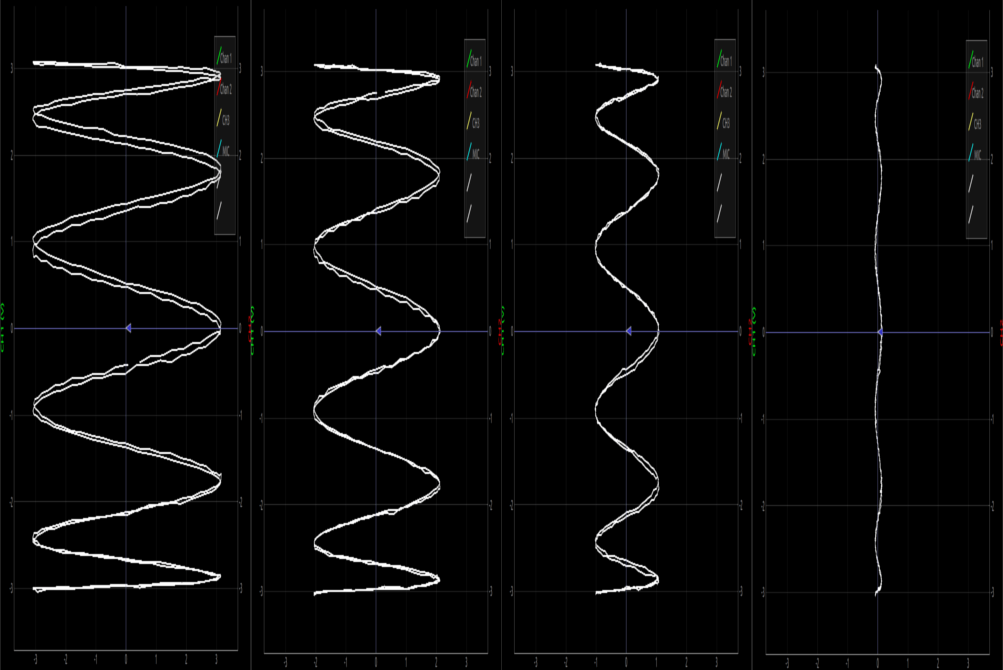
\includegraphics[width=14cm]{lissajous.jpg}};
\end{scope}

\draw[->,color=white] (-7,0) -- (7.5,0);

\def\xupper{1.7}
\xdef\xlower{-\xupper}
\draw[line width=0.7pt,color=white] (-7.1,\xupper) -- (7.5,\xupper);
\draw[line width=0.7pt,color=white] (-7.1,\xlower) -- (7.5,\xlower);


%\fill[color=red] (-6.315,0) circle[radius=0.08];
%\fill[color=red] (-5.92,0) circle[radius=0.08];
%\fill[color=red] (-5.2,0) circle[radius=0.08];
%\fill[color=red] (-4.13,0) circle[radius=0.08];
%\fill[color=red] (-2.85,0) circle[radius=0.08];
%\fill[color=red] (-1.37,0) circle[radius=0.08];
%\fill[color=red] (0.2,0) circle[radius=0.08];
%\fill[color=red] (1.73,0) circle[radius=0.08];
%\fill[color=red] (3.21,0) circle[radius=0.08];
%\fill[color=red] (4.52,0) circle[radius=0.08];
%\fill[color=red] (5.57,0) circle[radius=0.08];
%\fill[color=red] (6.32,0) circle[radius=0.08];
%\fill[color=red] (6.71,0) circle[radius=0.08];
%
\node[color=red] at (-6.315,0) [above left] {$x_0\mathstrut$};
\node[color=red] at (-5.92,0) [above right] {$x_1\mathstrut$};
\node[color=red] at (-5.2,0) [below right] {$x_2\mathstrut$};
\node[color=red] at (-4.13,0) [above right] {$x_3\mathstrut$};
\node[color=red] at (-2.85,0) [below right] {$x_4\mathstrut$};
\node[color=red] at (-1.37,0) [above right] {$x_5\mathstrut$};
\node[color=red] at (0.2,0) [above left] {$x_6\mathstrut$};
\node[color=red] at (1.73,0) [below left] {$x_7\mathstrut$};
\node[color=red] at (3.21,0) [above left] {$x_8\mathstrut$};
\node[color=red] at (4.52,0) [below left] {$x_9\mathstrut$};
\node[color=red] at (5.57,0) [above left] {$x_{10}\mathstrut$};
\node[color=red] at ({6.32+0.1},0) [below left] {$x_{11}\mathstrut$};
\node[color=red] at ({6.71},0) [below right] {$x_{12}\mathstrut$};

\def\xamplitude{6.57}
\def\yamplitude{1.66}

\begin{scope}[xshift=0.20cm]
\draw[color=red,line width=1pt] plot[domain=0:180,samples=1000]
	({\xamplitude*cos(\x)},{\yamplitude*cos(13*\x)});

\foreach \k in {0,...,13}{
	\pgfmathparse{(90+180*\k)/13}
	\xdef\winkel{\pgfmathresult}
	\fill[color=red] 
	({\xamplitude*cos(\winkel)},{\yamplitude*cos(13*\winkel)})
		circle[radius=0.08];
}

\node[color=white] at (0,{\yamplitude+0.4})
	{$\displaystyle \max \{\, l(x)\;|\; {-1}\le x \le 1 \} $};
\node[color=white] at (0,{-\yamplitude-0.4}) 
	{$\displaystyle \min \{\, l(x)\;|\; {-1}\le x \le 1 \} $};

\end{scope}

\end{tikzpicture}
\end{document}

